%\subsection{What is Event Coding}
\begin{frame}{A Hybrid Micro Tasking Framework for Event Coding}
Outline:
\begin{itemize}
    \item What is Event Coding?
    \item Necessity for a new Event Coder?
    \item System Framework
    \item Micro-tasks for Event Coding
\begin{itemize}
   \item Geo-coding
    \item Actor/Target Linking
    \item Temporal Resolution
    \item Event Detection
\end{itemize} 
    \item Performance
\end{itemize}
\end{frame}


\begin{frame}{What is Event Coding}
    \begin{figure}
        \centering
        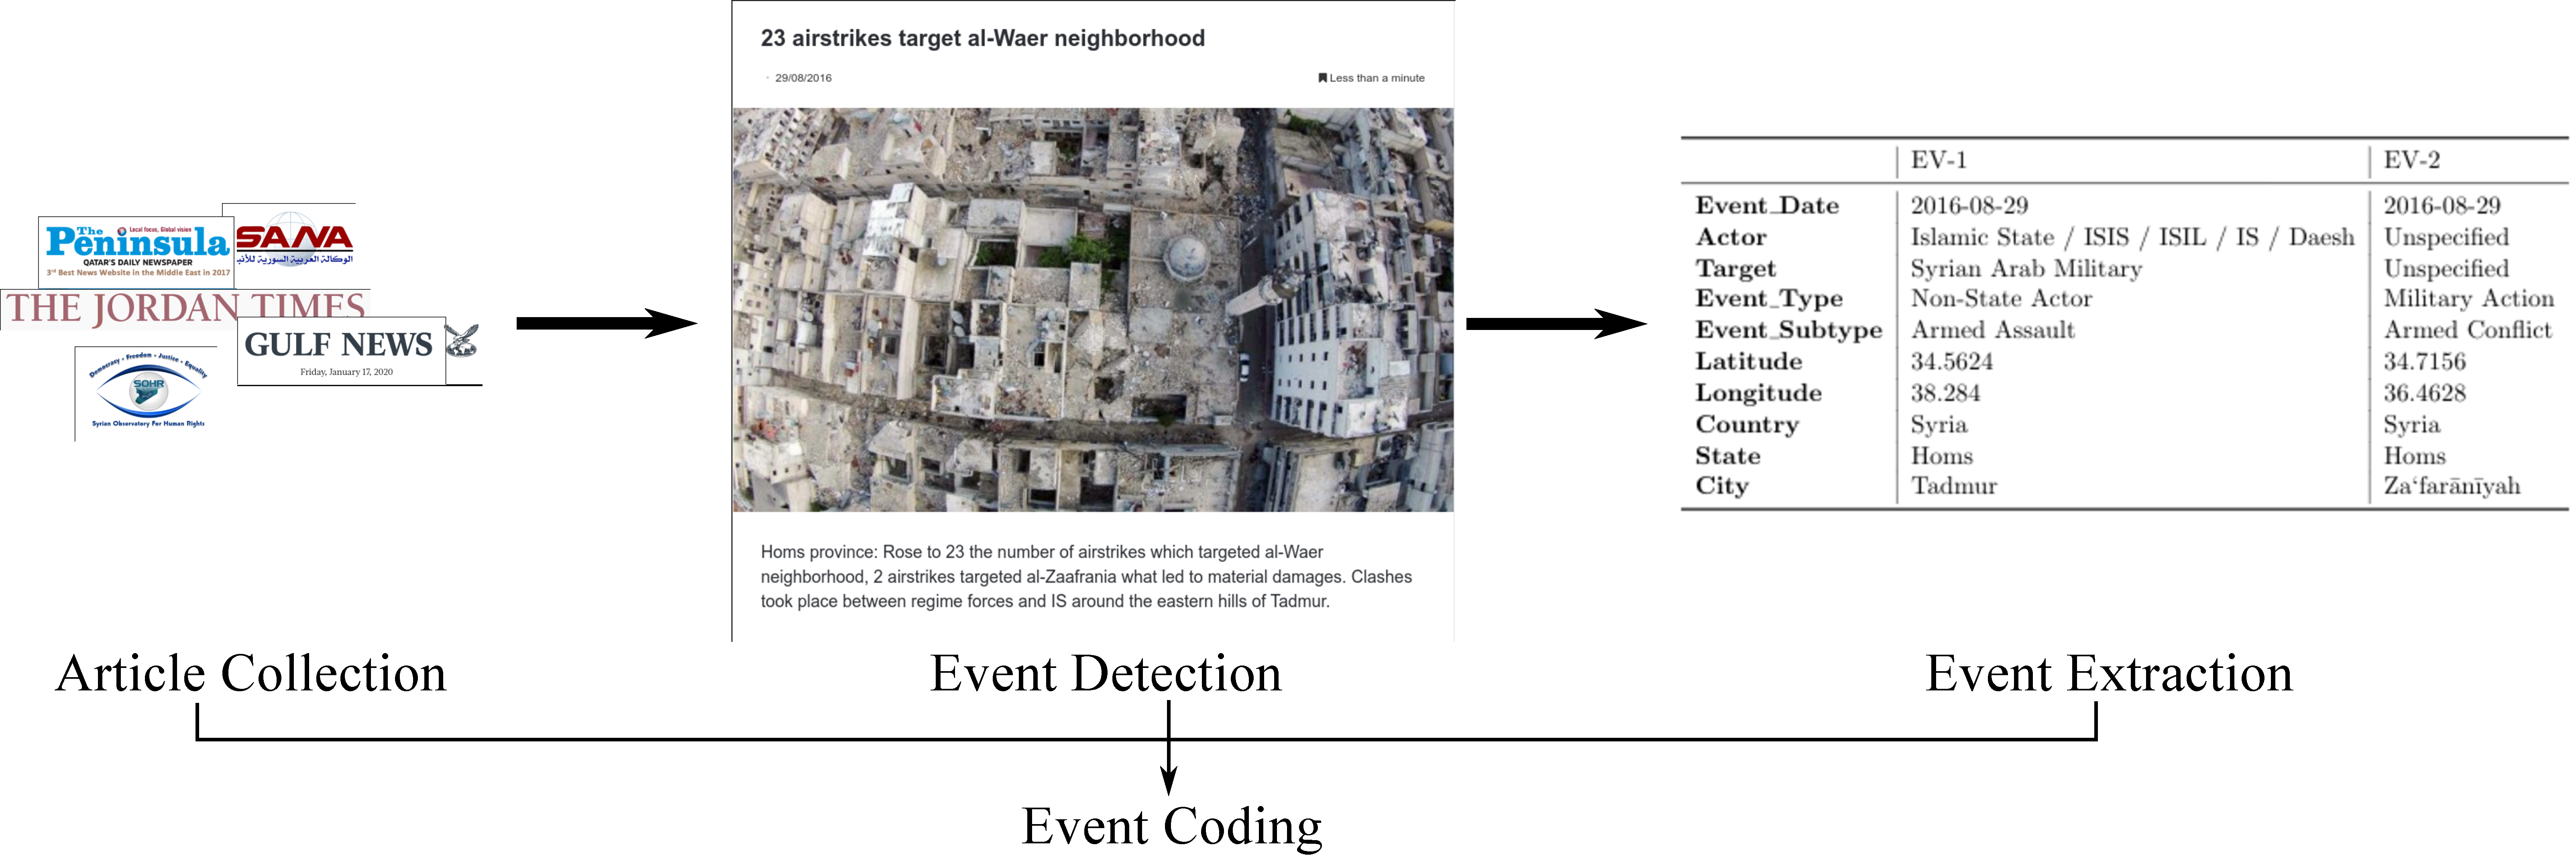
\includegraphics[width=\textwidth]{Problem2/figures/EventCoding_intro.pdf}
        \label{fig:my_label}
    \end{figure}
\end{frame}


%%\subsection{Necessity for a new Event Coder}
\begin{frame}{Necessity for a new Event Coder}
\begin{itemize}
    \item Manual event coders
    \begin{itemize}
        \item  High delay (OSI GSR (Goal Standard Report) had 1 month delay)
        \item High cost
    \end{itemize}
    \item Fully Automated Event coders 
    \begin{itemize}
        \item ICEWS~\cite{boschee2015icews}, GDELT~\cite{leetaru2013gdelt}
        \item Fixed dictionary (domain keywords and actors)
        \item fixed patterns for matching
        \item high duplicate levels
        \item Only English
    \end{itemize}
    \item Semi-Automatic event coders 
    \begin{itemize}
        \item EMBERS AutoGSR~\cite{saraf2016embers}
        \item Manual checking necessary for all fields and for all documents
    \end{itemize}
\end{itemize}
\end{frame}

%\subsection{Micro-tasks for Event Coding}
\begin{frame}{Micro-tasks for Event Coding}
    \begin{itemize}
    \item \textbf{Event Detection}: Classify if a news article is reporting an event of interest or not.
    \item \textbf{Geo-coding}: Identify and disambiguate location names from text
    \item \textbf{Actor / Target Linking}: Identify entities mentioned and link them to known actors. 
    \item \textbf{Temporal Reasoning}: Identify the exact date in which an event took place by resolving all direct and relative dates mentioned in the text.
    \item \textbf{Sub-type Identification}: This could be either the reason for the event (like Economic, Religious) in case of civil unrest or the kind of event (like bombing, hostage taking) in case of MANSA.
    \item \textbf{Event De-duplication}: Task of identifying if the current article refers to an already extracted event.
\end{itemize}
\end{frame}


%\subsection{System Framework}
\begin{frame}{System Framework}
    \begin{figure}
        \centering
        \includegraphics[width=\textwidth]{Problem2/figures/eventCoding_framework.pdf}
        \label{fig:my_label}
    \end{figure}
\end{frame}

%\subsection{Event Detection}
\begin{frame}{Event Detection}
Performed as a binary classification problem \\
\textbf{Uncertainty in Event Detection}
\begin{itemize}
    \item Base Classifier: Hierarchical Attention Network ~\cite{yang2016hierarchical}
    \item Uncertainty in Classification in literature
    \begin{itemize}
        \item Classification with reject option, Abstaining Classifiers, Selective classification 
        \item Methods can be broadly categorized into
        \begin{itemize}
            \item External model calibration - Platt scaling, Temperature scaling
            \item Ensemble learning - McDropout, Gaussian Process, Metric learning
            \item Learning a `K+1`th class for a K class problem - Deep.Abs Classifier, Evidential classification
        \end{itemize}
    \end{itemize}
    \end{itemize}
\end{frame}

\begin{frame}{Extraction using Dependency parsing}
\begin{itemize}
\small
    \item Extract events based on patterns on dependency tree
    \begin{itemize}
    \small
        \item ~\cite{predpatt},~\cite{pp-paper1},~\cite{reddy2017universal}
        \item universal dependency parser allows usage of same patterns for all languages
        \item All locations mentioned in the same sentence as the predicate-argument root is taken as Event location
    \end{itemize}    
\end{itemize}
\vspace{-1em}
\begin{figure}
    \centering
    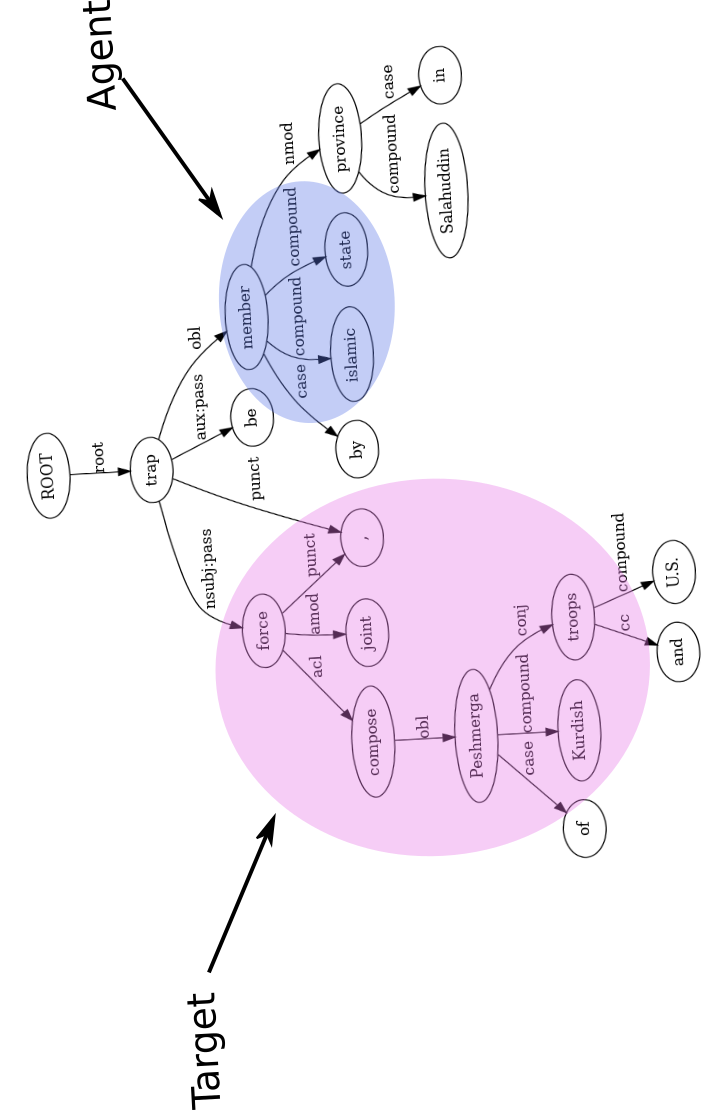
\includegraphics[width=0.35\textwidth, angle=-92]{Problem2/figures/depTree.png}
    \caption{Caption}
    \label{fig:my_label}
\end{figure}
\end{frame}

%\subsection{Geo-coding}
\begin{frame}{Geo-coding}
    Defined as the problem of identifying 1) mentions of placenames  in text and 2) grounding location names to geo-coordinates \\
    
    \begin{block}{Example}
    \alert{Baghdad Today} quoted the source saying that a bomb placed near a fish market in \alert{Wardiya, Madaen} exploded, killing one person and wounding four others
    \end{block}
\end{frame}

\begin{frame}{Geo-coding (contd.)}
\begin{itemize}
    \item Prior work is generally unsupervised and rule based
    \begin{itemize}
        \item Placenames are grounded to the most populous expansion (\textless Country, State, City \textgreater)
        \item Locations mentioned in same text share common ancestors or are nearby
    \end{itemize}
    \item Current state-of-the art - Mordecai~\cite{halterman2017mordecai}
    \begin{itemize}
        \item Neural network based model for inferring country for each placename
    \end{itemize}
\end{itemize}
\end{frame}

\begin{frame}{Supervised Geo-coding}

\begin{columns}
\column{0.6\textwidth}
Building Training Data

    \begin{itemize}
    \small
        \item Use only articles that contain events
        \item Extract placenames from article that have anyone grounding match to an event
        \item Expansion matching event location is labelled positive and rest negative
        \item Features
        \begin{itemize}
            \item Frequency of country in expansions of all names in text
            \item Relative Population 
            \item Mean, Min token distance to Placename having an expansion from the same country
            \item Token distance to the next nearest Placename (before and after)
        \end{itemize}
    \end{itemize}


\column{0.4\textwidth}
\begin{figure}
    \centering
    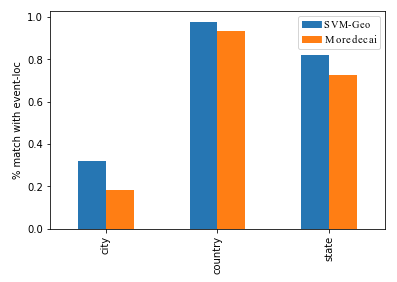
\includegraphics[width=\textwidth]{Problem2/figures/Geo_metrics.png}
    \label{fig:my_label}
\end{figure}
\end{columns}

\end{frame}

\begin{frame}{Uncertainty in Geo-coding}
\begin{itemize}
    \item Approximate locations
    \begin{itemize}
        \item Percentage of Approximate locations is 27.81\% (4400 events, 3053 documents, 5 month period)
        \begin{block}{}
         Three people killed by a landmine explosion in their car in the \alert{rough neighborhood of Jaroud Arsal} left behind by terrorists.
        \end{block}
        \item Uncertainty in Location disambiguation (Example on next slide)
    \end{itemize}
\end{itemize}
\end{frame}

\begin{frame}{Uncertainty in Geo-coding}
\begin{figure}
    \centering
    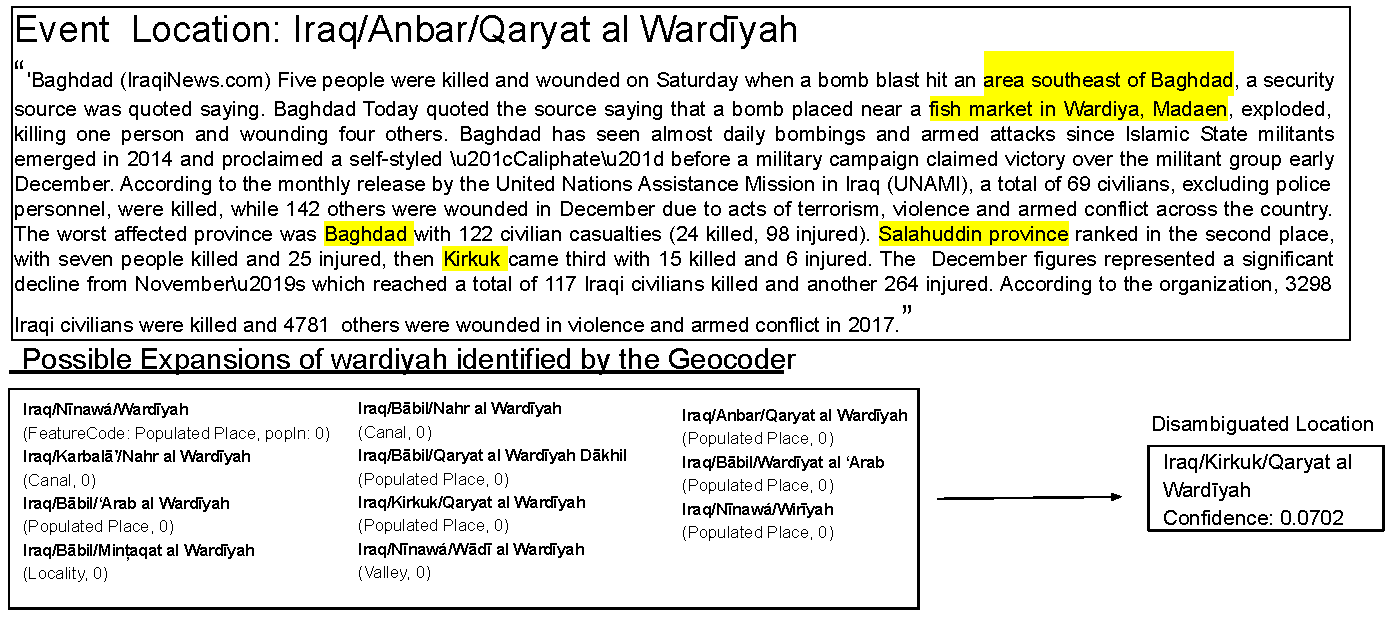
\includegraphics[width=1\textwidth]{Problem2/figures/Geo_uncertainty.pdf}
    \label{fig:my_label}
\end{figure}
\end{frame}

%\subsection{Actor/Target Linking}
\begin{frame}{Actor/Target Linking}
Categorized into two kinds
    \begin{itemize}
        \item Specific Nouns (like Jordanian Police, Democratic Union Party / PYD)
        \begin{itemize}
            \item Fuzzy token similarity for matching
        \end{itemize}
        \item Generic Nouns (Weapon/Equipment, Vehicle, Checkpoint)
        \begin{itemize}
            \item Expand keyword list
            \begin{itemize}
                \item High similarity neighbors from word embedding
                \item Example: Airstrike, bombardment
                \item Words that share similar hypernyms / hyponyms / synsets from Wordnet 
                \item Example: Builders, Contractors, Constructor
            \end{itemize}
        \end{itemize}
    \end{itemize}
\end{frame}

\begin{frame}{Uncertainty in Actor/Target Linking}
\begin{block}{EVENT:(Location) Syria-Aleppo-Rā‘il,  (Actor) Al-Moatasim / Al-Moatasim Brigade,  2018-05-23,  (Target) Unspecified}
\small
``The town of Al-Ra’I on the border with Turkey, which is controlled by the factions operating within the Turkish-backed operation of the “Euphrates Shield”, witnessed tension between a faction operating in the area and the free police operating in the town, and in the details obtained by the Syrian Observatory of Human Rights; the town is witnessing a state of alertness and tension, followed a fight took place between \alert{Al-Muntasir Brigade} against the free police, in the market of the town... ''
\end{block}

\begin{itemize}
    \item New Actor
    \item Unknown alias of an existing actor
\end{itemize}

\end{frame}

%\subsection{Temporal Resolution}
\begin{frame}{Temporal Resolution}
Broadly defined as the task of converting relative temporal expressions like `two days ago' into exact dates
\begin{itemize}
    \item TIMEN~\cite{timen}
    \item Heideltime~\cite{heideltime}
        \begin{itemize}
            \item Larger number of language classes
            \item Covers more temporal patterns
        \end{itemize}
\end{itemize}
\end{frame}



%\subsection{Sub-type Identification}
% \begin{frame}{Event Sub-type identification}
% \begin{itemize}

%     \item Word-net expansion and classification
%     \end{itemize}
% \end{frame}



%\subsection{Performance Metrics}
\begin{frame}{Performance Metrics}
Train Data: Upto May 2018, Validation: June 2018, Test - August-October 2018
\begin{itemize}
    \item \textbf{Event Detection Performance Metrics}
    \begin{itemize}
        \item Precision/Recall/F1 metrics
        \item Risk-Coverage Curve
        \begin{itemize}
            \item Risk is percentage of false classifications (False Positives + False Negatives)
            \item Coverage is percentage of data remaining after removing low-confidence documents
        \end{itemize}
    \end{itemize}
\item \textbf{Event Encoding Performance Metrics}
    \begin{itemize}
        \item \textbf{Quality Score:}  The components of QS are:
            \begin{enumerate}
                \item Actor score (AS)
                \item Target Target score (TTS)
                \item Target Status score (TS)
                \item Location score (LS): $(1 – Dist/300)$
                \item Event Sub-type score (ES)
                \item Date score (DS): $max(diff, 7)/7$
            \end{enumerate}
         \item \textbf{Macro and Micro averages}
    \end{itemize}    
\end{itemize}
\end{frame}


\begin{frame}{Event Detection Performance}
\textbf{English}
\begin{table}
\small
    \centering
   \begin{tabular}{lrrrr}
\toprule
{} &  Precision &  Recall &    F1-score &  Support \\
\midrule
No-event            &  0.97 &   0.95 &  0.96 &   15843 \\
Event               &  0.75 &   0.84 &  0.79 &   2760 \\
micro avg           &  0.93 &   0.93 &  0.93 &   18603 \\
macro avg           &  0.86 &   0.90 &  0.88 &   18603 \\
weighted avg        &  0.94 &   0.93 &  0.94 &   18603 \\
\bottomrule
\end{tabular}
    \label{tab:engDetection}
\end{table}

\textbf{Arabic}
\begin{table}
\small
    \centering
   \begin{tabular}{lrrrr}
\toprule
{} &  Precision &  Recall &    F1-score &  Support \\
\midrule
No-event            &  1.0 &  1.00 &  1.00 &  28643 \\
Event               &  1.0 &  0.36 &  0.53 &   73 \\
micro avg           &  1.0 &  1.00 &  1.00 &  28716 \\
macro avg           &  1.0 &  0.68 &  0.76 &  28716 \\
weighted avg        &  1.0 &  1.0  &  1.00 &  28716 \\
\bottomrule
\end{tabular}
    \label{tab:arDetection}
\end{table}
\end{frame}

\begin{frame}{Performance of fully Automated system}
\begin{columns}
\column{0.3\textwidth}
\textbf{Macro-Avg}: Extracted events in a document are only evaluated against the ground-truth events in that document
\column{0.7\textwidth}
        \begin{table}
    \centering
    \begin{tabular}{l|r|r}
    \toprule
                 Metrics &    Macro-avg &    Micro-avg \\
    \midrule
                   \#docs &   888 &   888 \\
     \# GroundTruthEvents &  2039 &  2039 \\
       \# ExtractedEvents &  1981 &  1981 \\
             Actor Score &     0.373888 &     0.602880 \\
              Date Score &     0.940764 &     0.840740 \\
     Event Subtype Score &     0.449895 &     0.680532 \\
          Location Score &     0.866620 &     0.800837 \\
     Target Target Score &     0.662297 &     0.677204 \\
     Target Status Score &     0.590778 &     0.828618 \\
               Precision &     0.691522 &     0.949447 \\
                  Recall &     0.720177 &     0.891757 \\
           Quality Score &     2.774264 &     2.999131 \\
    \bottomrule
    \end{tabular}
    \label{tab:mlPerformance}
    \end{table}
\end{columns}
\end{frame}

\begin{frame}{System Performance after Actor Grouping}
\begin{columns}
\column{0.5\textwidth}
\begin{itemize}
    \item Group different state actors of a given country into one entity
    \item Example: Following are grouped into Iraqi State Actors
    \begin{itemize}
        \item Iraq Security Forces
        \item Iraqi Intelligence Service
        \item Iraqi Police
        \item Baghdad International Airport Security
        \item Iraqi Military
        \item Iraqi Special Forces
    \end{itemize}
\end{itemize}
\column{0.5\textwidth}
\begin{table}
\centering
\begin{tabular}{lrr}
\toprule
       Metric &    Macro-avg &    Micro-avg \\
\midrule
\textbf{After} & & \\
       AS &     0.551 &     0.727 \\
       QS &     2.892 &     3.087 \\
       \midrule
       \textbf{Before} & & \\
        AS &     0.373 &     0.602 \\
        QS &     2.774 &     2.999 \\
\bottomrule
\end{tabular}
\label{tab:mlgrouped}
\end{table}
\end{columns}
\end{frame}

\begin{frame}{Characterization of human annotators}
\begin{figure}
     \centering
     \begin{subfigure}[b]{0.5\textwidth}
         \centering
         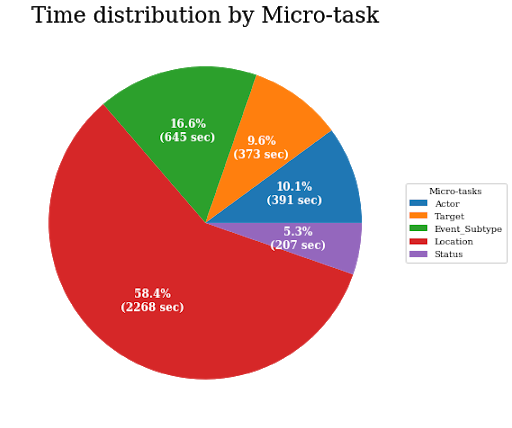
\includegraphics[width=\textwidth]{Problem2/figures/micro_task_timings.png}
     \end{subfigure}%
     \hfill
     \begin{subfigure}[b]{0.5\textwidth}
         \centering
         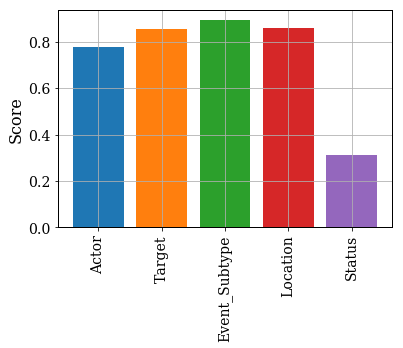
\includegraphics[width=\textwidth]{Problem2/figures/micro_task_performance.png}
     \end{subfigure}
\end{figure}
    
\end{frame}

% \begin{frame}{Uncertainty characterization event detection model}
% \begin{col}
% \begin{figure}
%     \centering
%     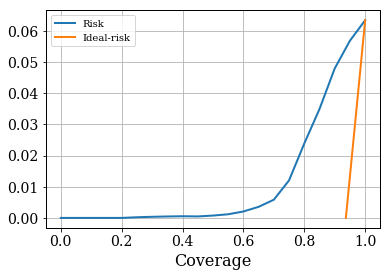
\includegraphics[width=0.45\textwidth]{Problem2/figures/english_riskCoverage.png}
% \end{figure}
% \end{frame}

\begin{frame}{Number of Documents sent for supervision}
\begin{table}
    \centering
    \small
    \begin{tabular}{l|r}
    \toprule
       \textbf{Micro-Task}  & \textbf{\#Abstained Documents} \\
    \midrule
       Event Detection &  1936 / 57401 (3.00\%) \\
       Location  & 307/2137 (14.3\%) \\
       Actor/Target & 1002/2137 (46.8\%) \\
       All (Location, Actor, Subtype) & 320/2137 (14.9\%) \\
    \bottomrule
    \end{tabular}
    \caption{Documents sent for human supervision}
    \label{tab:abstPerMicro}
\end{table}
\end{frame}

\begin{frame}{Performance of Hybrid System}
    \begin{table}[]
    \centering
    \begin{tabular}{lrr}
\toprule
              Metric &    Macro-avg &    Micro-avg \\
\midrule
               \#docs &  2137 &  2137 \\
 \# GroundTruthEvents &  4265 &  4265 \\
   \# ExtractedEvents &  4239 &  4239 \\
         Actor Score &     0.621032 &     0.755090 \\
          Date Score &     0.952899 &     0.878390 \\
 Event Subtype Score &     0.539359 &     0.646776 \\
      Location Score &     0.926107 &     0.838040 \\
 Target Target Score &     0.680881 &     0.703337 \\
 Target Status Score &     0.727046 &     0.828054 \\
           Precision &     0.791948 &     0.946720 \\
              Recall &     0.819668 &     0.915887 \\
       Quality Score &     3.121909 &     3.161470 \\
\bottomrule
\end{tabular}
    \label{tab:hybridPerf}
\end{table}
\end{frame}

\begin{frame}{Comparison with ICEWS}
CAMEO Codes used: 1) 15 - Exhibit Military Posture,  2) 18 - Assault
\begin{figure}
    \centering
    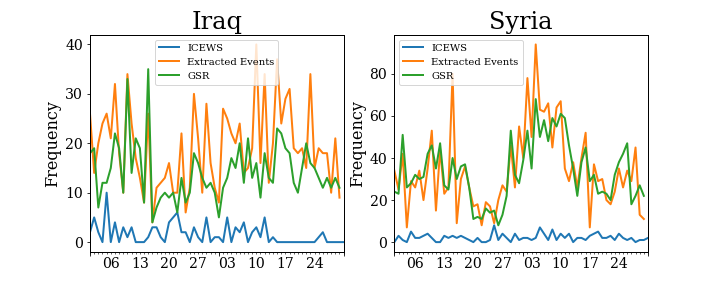
\includegraphics[width=\textwidth]{Problem2/figures/ICEWS_comparison.png}
\end{figure}
    
\end{frame}

\begin{frame}{Takeaways}
\begin{itemize}
    \item Automated methods perform well in identifying Location, Date
    \item Human supervision necessary for Actor/Target identification
    \item Contributions
    \begin{itemize}
        \item Improved geo-coding performance
        \item Automated approaches for keyword expansion
        \item language agnostic extraction
    \end{itemize}
\end{itemize}
    
\end{frame}

